\documentclass{article}
\usepackage{adjustbox}
\usepackage{float}
\usepackage{textcomp}
\usepackage{graphicx}
\graphicspath{{images/}}
\usepackage{booktabs}
\usepackage{color}
\usepackage{verbatim}
\usepackage{listings}
\usepackage{underscore}
\setcounter{secnumdepth}{5}
\usepackage[bookmarks=true]{hyperref}
\author{Roberto Clapis (841859), Erica Stella (854443)} 
\date{\today}
\title{Politecnico di Milano
	\\A.A. 2015\@-\@2016
	\\Software Engineering 2: ``myTaxiService''
	\\\textbf{P}roject \textbf{P}lan}
\hypersetup{pdftitle={Project Plan},    % title
	pdfauthor={Roberto Clapis, Erica Stella},                     % author
	pdfsubject={Project Plan},                        % subject of the document
	pdfkeywords={TeX, LaTeX, taxi, PP, SoftwareEngineering2}, % list of keywords
	colorlinks=true,       % false: boxed links; true: colored links
	linkcolor=black,       % color of internal links
	citecolor=blue,       % color of links to bibliography
	filecolor=black,        % color of file links
	urlcolor=purple,        % color of external links
}
\begin{document}
\maketitle
\begin{center}
	
\includegraphics{polimi-logo}
\end{center}
\clearpage
\tableofcontents
\clearpage
\section{Introduction}
This document describes the project plan for myTaxiService application.
It presents an analysis of the expected size and effort required 
for the implementation phase calculated respectively with the Function
Points and COCOMO. Then it presents the available resources and how 
they will be allocated to the project tasks and, in the end, it
discusses the possible risks this project might encounter and the
associated recovery actions.
%TODO finire
\section{Size and Effort Estimation}
\subsection{Size Estimation - Function Points}
\begin{center}
	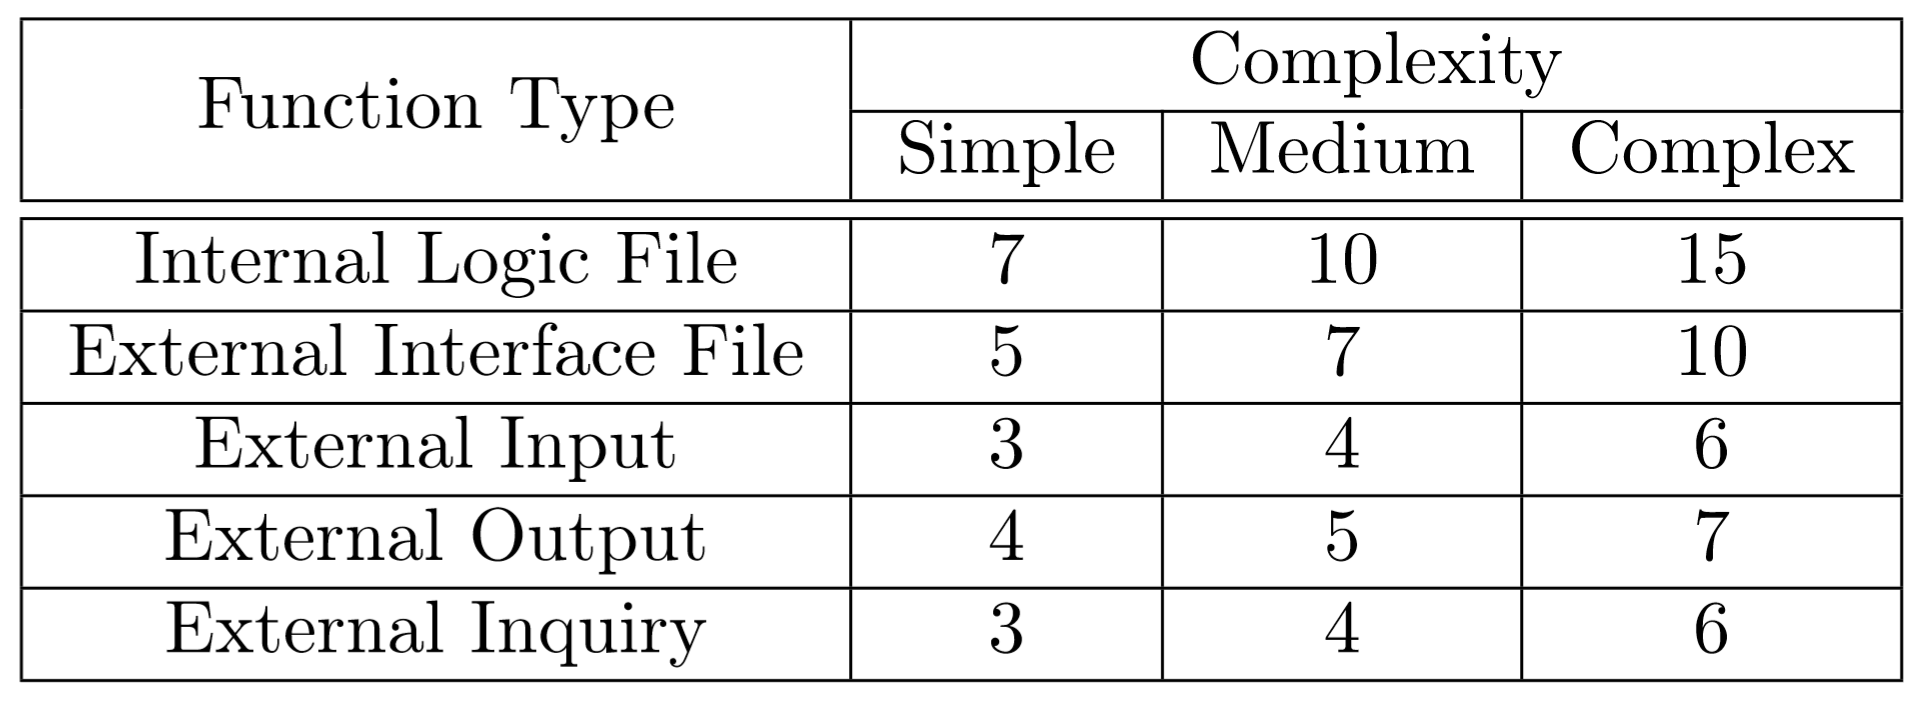
\includegraphics[width = 0.8\textwidth]{FP}
\end{center}
\subsection{Effort Estimation - COCOMO}
\section{Resource Allocation}
\subsection{Tasks}
RASD:
\begin{itemize}
	\item
\end{itemize}
Design Document:
\begin{itemize}
	\item
\end{itemize}
Code Inspection:
\begin{itemize}
	\item
\end{itemize}
Integration Test Plan Document:
\begin{itemize}
	\item 
\end{itemize}
\section{Risks}
\end{document}